\documentclass[a4paper,11pt]{article}

\usepackage[english]{babel} 
\usepackage[utf8]{inputenc}
\usepackage[cyr]{aeguill}
\usepackage{stmaryrd}

\usepackage{lmodern} %Type1-font for non-english texts and characters
\usepackage{caption}
\usepackage{subcaption}

\usepackage{graphicx}
\usepackage{hyperref}

\usepackage{epstopdf}


%\hypersetup{	
%colorlinks=true,   %colorise les liens 
%breaklinks=true,  %permet le retour à la ligne dans les liens trop longs 
%urlcolor= blue,    %couleur des hyperliens 
%linkcolor= black, %couleur des liens internes 
%citecolor=black,	 %couleur des références 
%pdftitle={Compte rendu \emph{Traitement numérique du signal}, %informations apparaissant dans 
%pdfauthor={Mélisande Zonta}, %les informations du document 
%pdfsubject={Projet TNS2}	%sous Acrobat. 
%} 

%% Math Packages 
\usepackage{amsmath}
\usepackage{amsthm}
\usepackage{amsfonts}
\usepackage{amssymb}
\usepackage{mathrsfs}
\usepackage{pst-all}
\usepackage{lscape}
\usepackage{pdfpages}
\usepackage{mathabx}


\usepackage{color, colortbl}
\definecolor{lightgray}{gray}{0.85}
\usepackage{multirow}
\usepackage[Algorithme]{algorithm}
\usepackage[noend]{algpseudocode}
\usepackage{tikz}

%\renewcommand{\algorithmicdo}{\textbf{faire}}
%\renewcommand{\algorithmicwhile}{\textbf{tant que}}


\usepackage{a4wide} %%Smaller margins = more text per page.
\usepackage{fancyhdr} %%Fancy headings

\setcounter{secnumdepth}{5}
\setcounter{tocdepth}{5}


\DeclareMathOperator*{\argmax}{arg\,max}
\DeclareMathOperator*{\argmin}{arg\,min}
\graphicspath{{/Users/melisandezonta/Documents/Documents/GTL_courses_second_semester/Computer-Vision/PS0-all/PS0-images/}}

\begin{document}

%\pagestyle{fancy}

\begin{titlepage}
\vspace*{\stretch{1}}

\begin{center}

\includegraphics[scale=0.4]{GT_logo.jpeg}
\end{center}
\vspace*{\stretch{1}}
\hrulefill
\begin{center}\bfseries\huge
   Computer Vision \\
   CS 6476 , Spring 2018\\
   \end{center}
  \begin{center}\bfseries\large
     PS 0\\
    \hrulefill
\end{center}
%\hfill
\vspace*{1cm}
\begin{minipage}[t]{0.6\textwidth}
  \begin{flushleft} \large
    \emph{Supervisor : }\\
    Cedric Pradalier \\
  \end{flushleft}
\end{minipage}
\begin{minipage}[t]{0.3\textwidth}
  \begin{flushright} \large
    \emph{Author :} \\
    Melisande Zonta \\
  \end{flushright}
\end{minipage}
\vspace*{\stretch{2}}
\begin{flushright}
       Le \today 
\end{flushright} 
\end{titlepage}

\tableofcontents
\clearpage

\section{Input Images}

\begin{figure}[H]
\centering
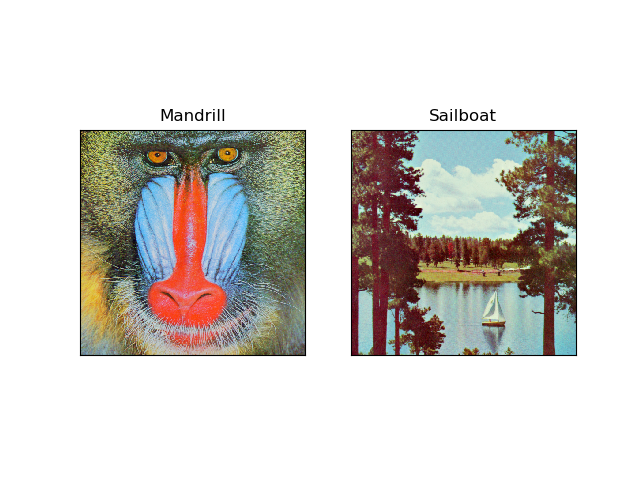
\includegraphics[width = 1\textwidth]{input_images.png}
 \caption{Input images}
\label{input_images}
\end{figure}

\section{Color planes}
\subsection{Swap the red and blue pixels }

\begin{figure}[H]
\centering
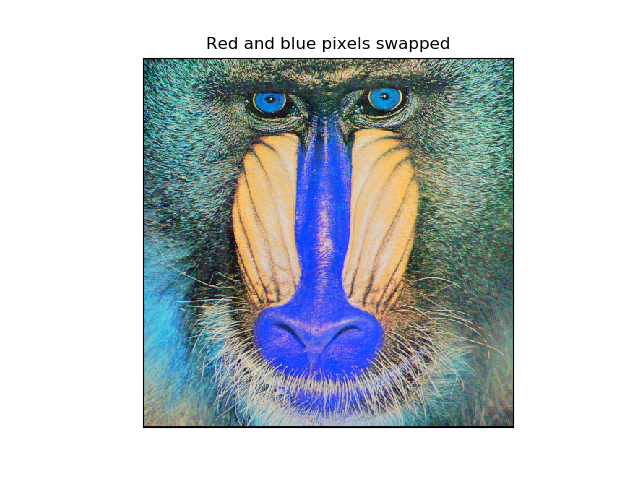
\includegraphics[width = 1\textwidth]{ps0-2-a.png}
 \caption{ps0-2-a : Red and blue pixels swapped}
\label{ps0-2-a}
\end{figure}

\subsection{Creation of a monochrome image (M1g)}

\begin{figure}[H]
\centering
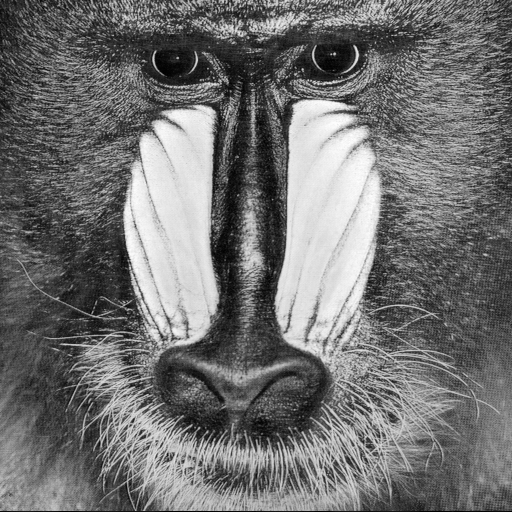
\includegraphics[width = .5\textwidth]{ps0-2-b.png}
 \caption{ps0-2-b : Green channel selection}
\label{ps0-2-b}
\end{figure}

\subsection{Creation of a monochrome image (M1r) }

\begin{figure}[H]
\centering
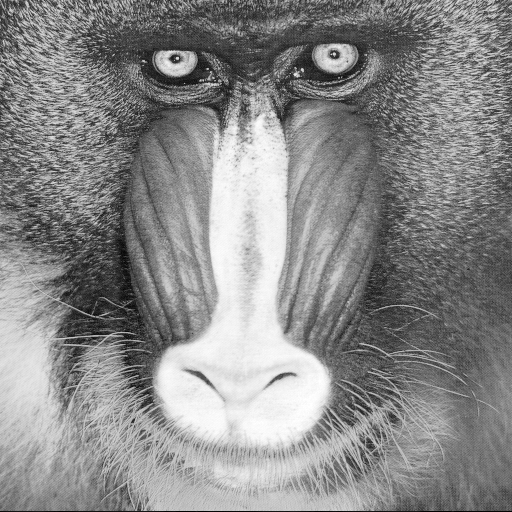
\includegraphics[width = .5\textwidth]{ps0-2-c.png}
 \caption{ps0-2-c : Red channel selection}
\label{ps0-2-c}
\end{figure}

\subsection{Comparison }

The results seem to be more or less as accurate with the red or the green channels. Nevertheless, we could say that the red monochrome image is better since the human brain is the more sensible to red light.

\section{Replacement of pixels}
\subsection{Selection and insertion of a ROI}

 \begin{figure}[H]
\begin{center}
\begin{tabular}{cc}
	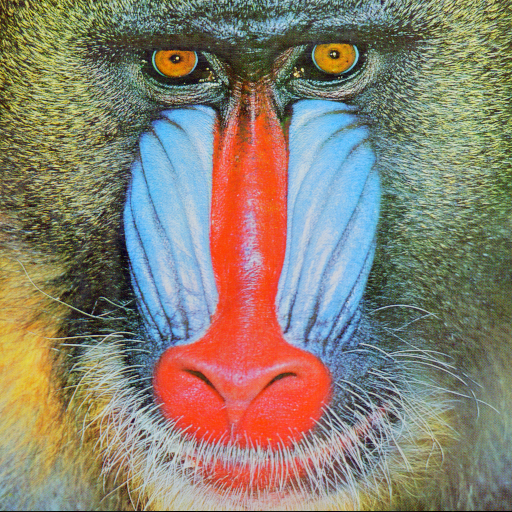
\includegraphics[height=.3\textwidth]{ps0-3-a-1.png}&
	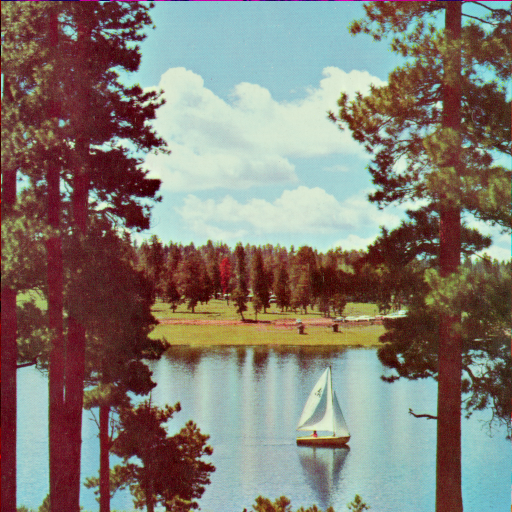
\includegraphics[height=.3\textwidth]{ps0-3-a-2.png}\\
	a&b\\
	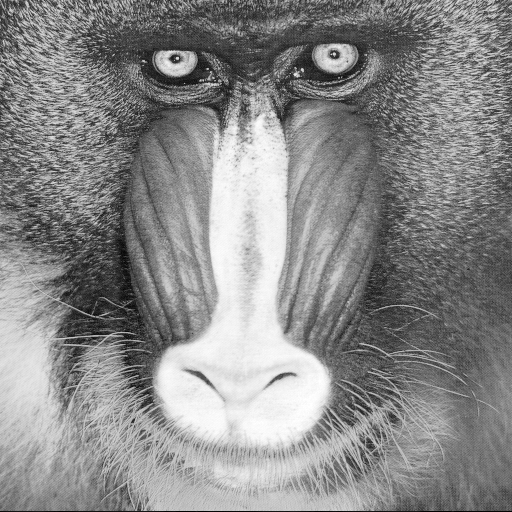
\includegraphics[height=.3\textwidth]{ps0-3-a-3.png}&
	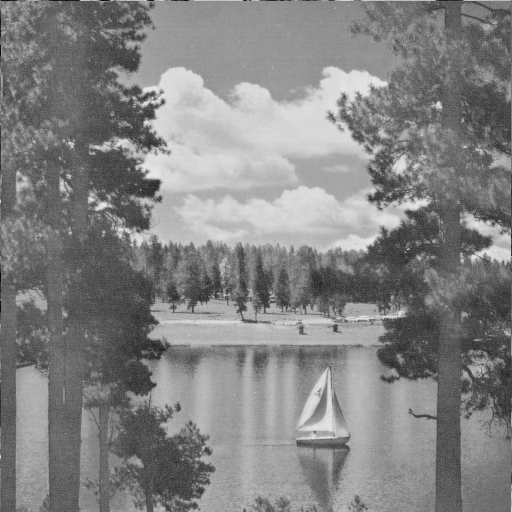
\includegraphics[height=.3\textwidth]{ps0-3-a-4.png}\\
	c&d\\
	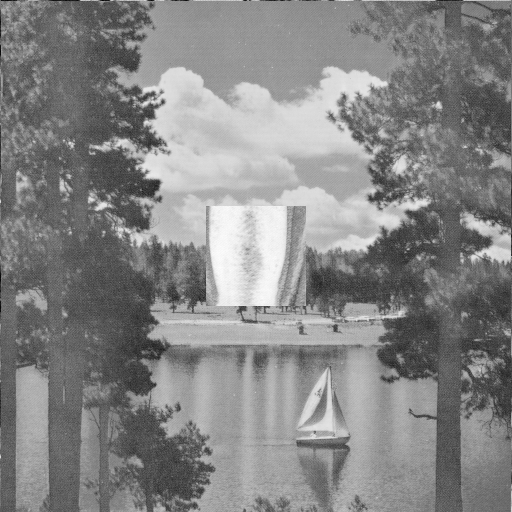
\includegraphics[height=.3\textwidth]{ps0-3-a-5.png}\\
	e
\end{tabular}
\end{center}
\caption{ 
\textit{a}. ps0-3-a-1 : Original Image 1. \textit{b}. ps0-3-a-2 : Original Image 2. \\
\textit{c}. ps0-3-a-3 : Red monochrome Image 1. \textit{d}. ps0-3-a-4 : Red monochrome Image 2.\\
\textit{e}. ps0-3-a-5 : Insertion of the inner square of the image 1 into the image 2.}
\label{ps0-3-as}
\end{figure}

\section{Arithmetic and Geometric operation}
\subsection{Determination of some statistical parameters}

\begin{enumerate}
\item The minimal pixel value of the green monochrome version of the image 1 is :  0.\\
\item The maximal pixel value of the green monochrome version of the image 1 is :  236.\\
\item The mean of the green monochrome version of the image 1 is :  128.858776093.\\
\item The standard deviation deviation of the green monochrome version of the image 1 is :  47.7705860899\\
\end{enumerate}
Those results seem consistent in value with the range [0,255] since the average is the half of the range.
\subsection{Normalization of the image}

 \begin{figure}[H]
\begin{center}
\begin{tabular}{cc}
	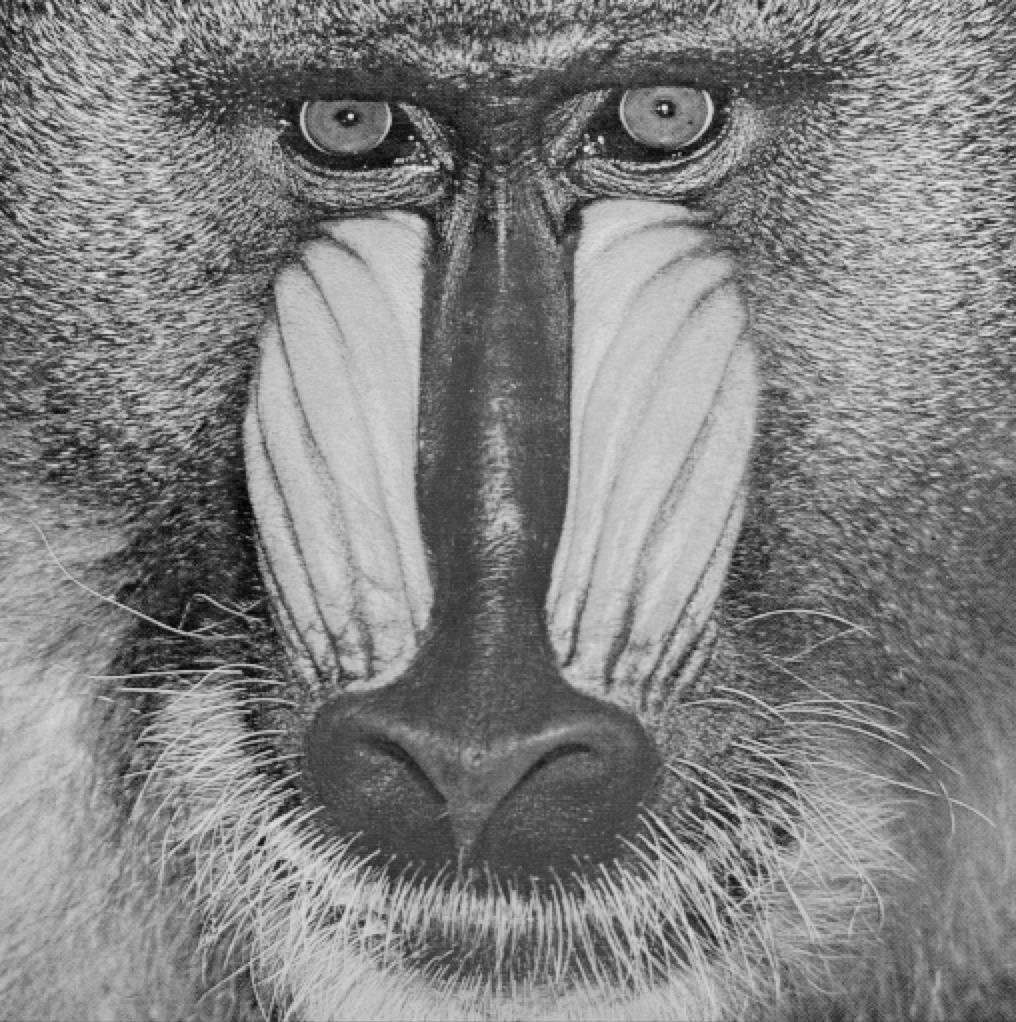
\includegraphics[height=.3\textwidth]{ps0-4-b-1.png}&
	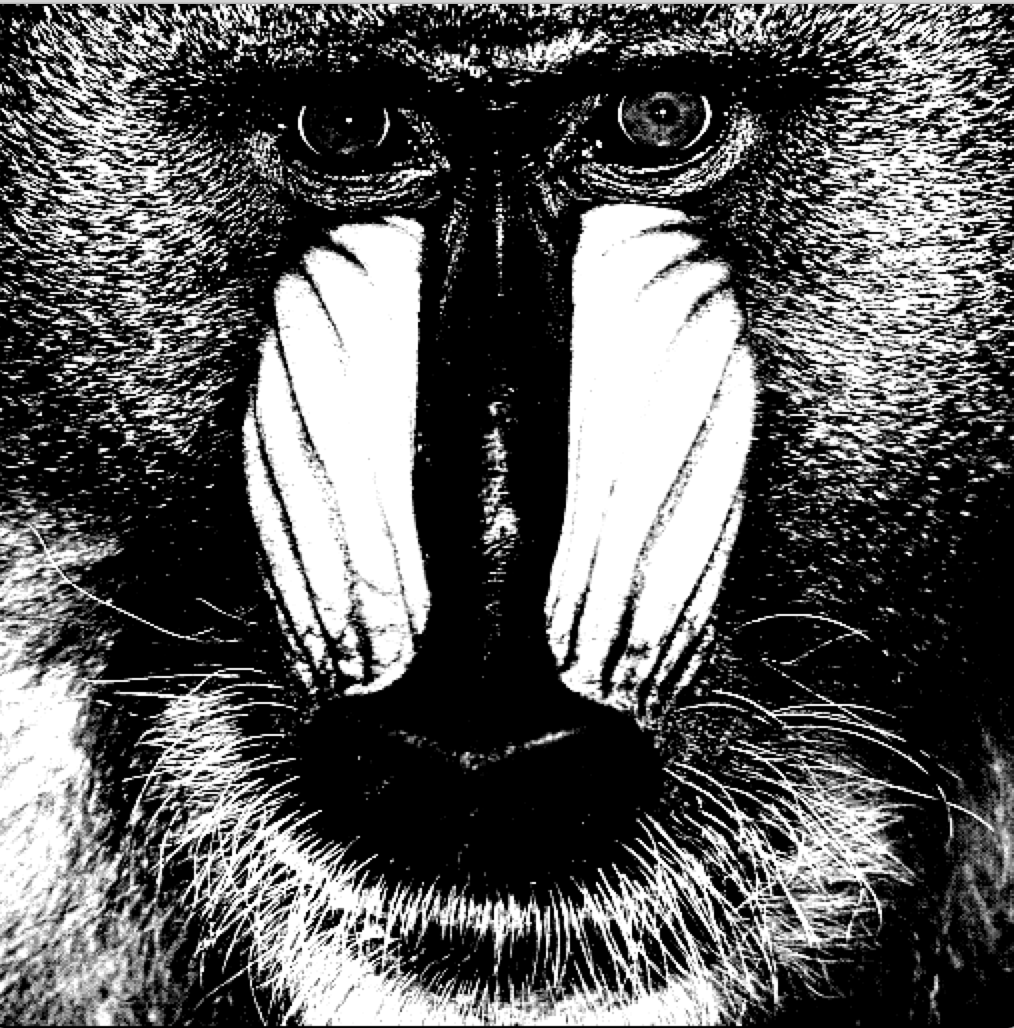
\includegraphics[height=.3\textwidth]{ps0-4-b-2.png}\\
	a&b\\
	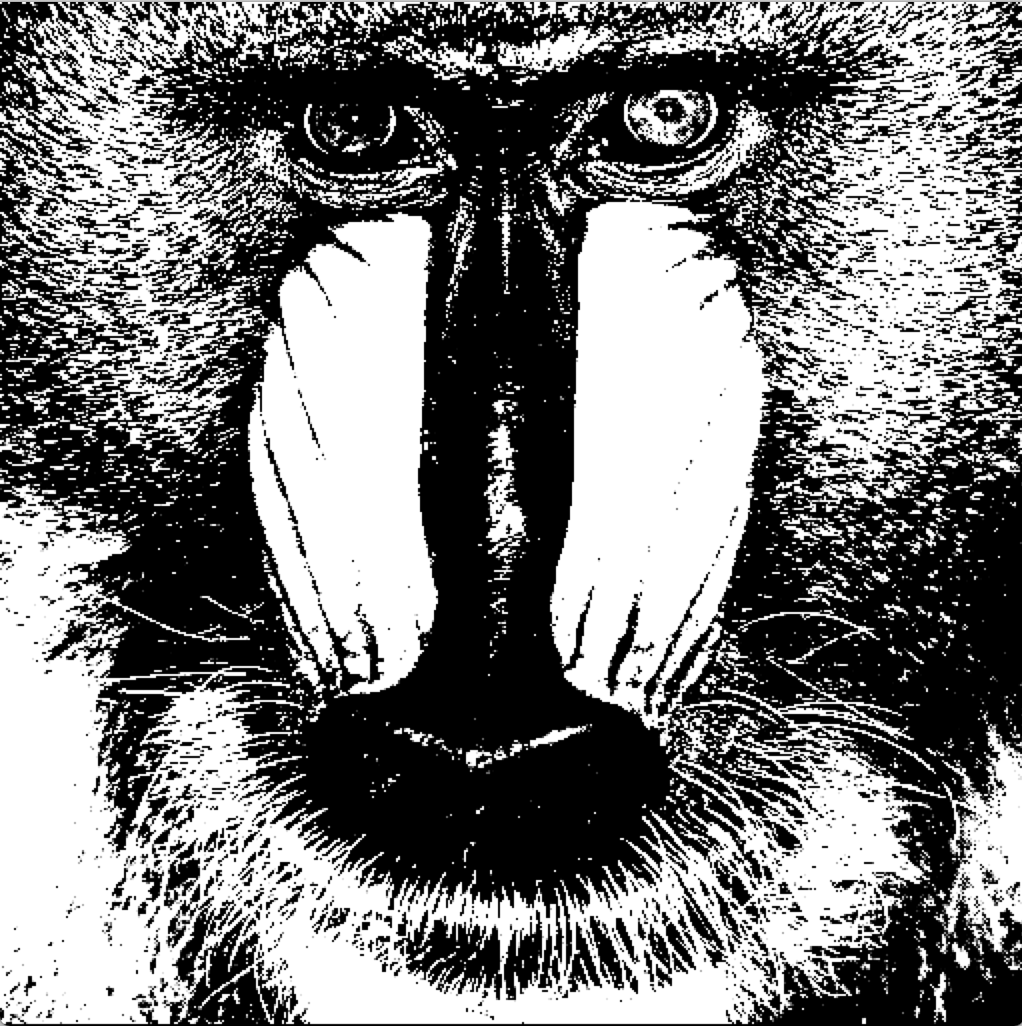
\includegraphics[height=.3\textwidth]{ps0-4-b-3.png}&
	
\includegraphics[height=.3\textwidth]{ps0-4-b-4.png}\\
	c&d\\
\end{tabular}
\end{center}
\caption{ 
\textit{a}. ps0-4-b-1 : Original green monochrome image \textit{b}. ps0-4-b-1 : Normalized image\\
\textit{c}. ps0-4-b-1 : Rescaled image  \textit{d}. ps0-4-b-1 : Final image}
\label{ps0-4-b}
\end{figure}

\subsection{Shift}

 \begin{figure}[H]
\begin{center}
\begin{tabular}{cc}
	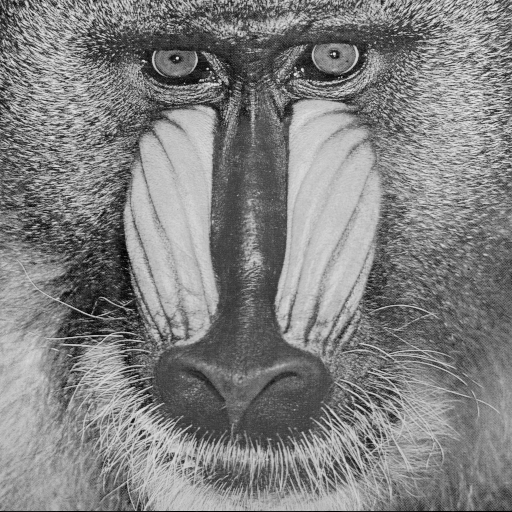
\includegraphics[height=.3\textwidth]{ps0-4-c-1.png}&
	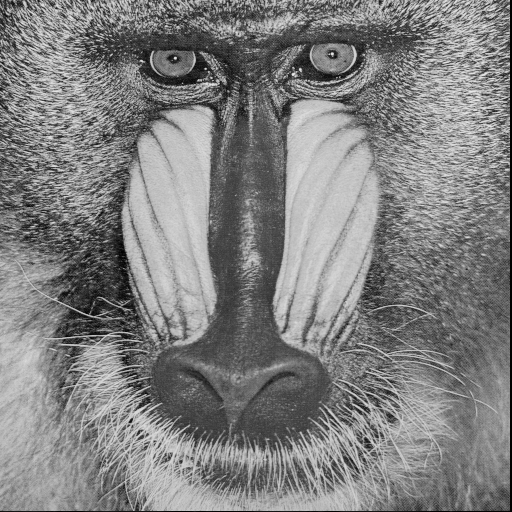
\includegraphics[height=.3\textwidth]{ps0-4-c-2.png}\\
	a&b\\
\end{tabular}
\end{center}
\caption{ 
\textit{a}.ps0-4-c-1 : Original green monochrome image . \textit{b}. ps0-4-c-2 : Shifted Image.}
\label{ps0-4-c}
\end{figure}

\subsection{Subtraction of the shifted version and the original version}

 \begin{figure}[H]
\begin{center}
\begin{tabular}{cc}
	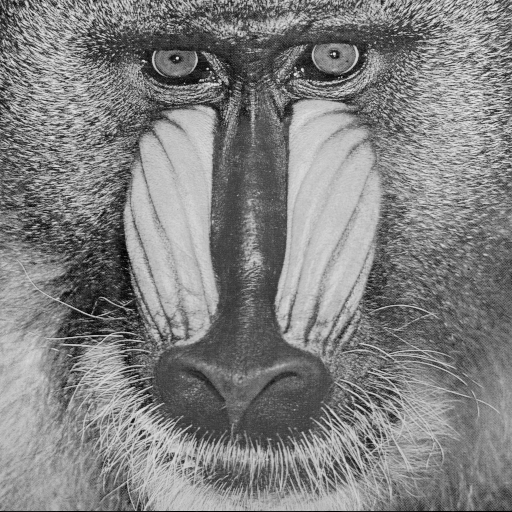
\includegraphics[height=.3\textwidth]{ps0-4-d-1.png}&
	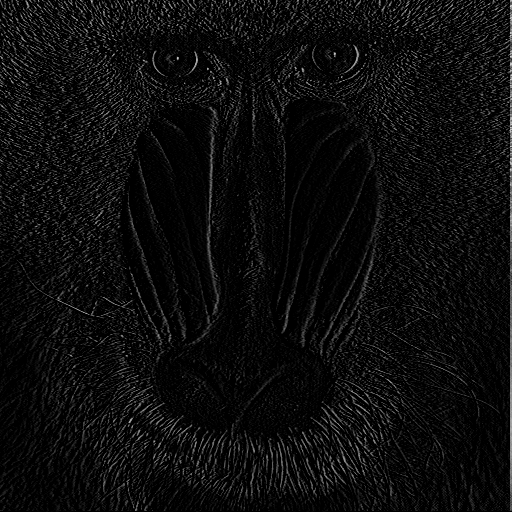
\includegraphics[height=.3\textwidth]{ps0-4-d-2.png}\\
	a&b\\
\end{tabular}
\end{center}
\caption{ 
\textit{a}. ps0-4-d-1 : Original green monochrome image . \textit{b}. ps0-4-d-2 : Subtracted Image.}
\label{ps0-4-d}
\end{figure}

\section{Noise}
\subsection{Noise introduction in the green monochrome image}

 \begin{figure}[H]
\begin{center}
\begin{tabular}{cc}
	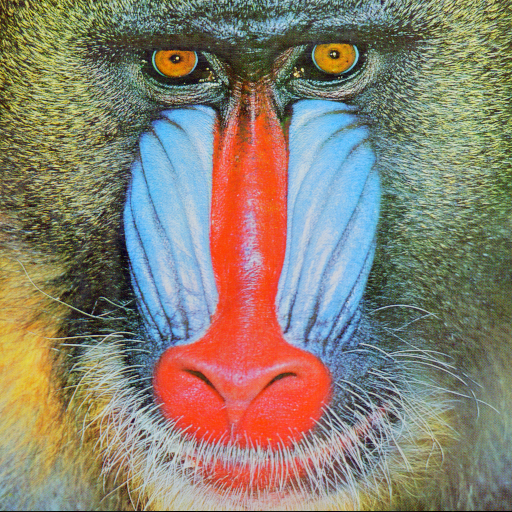
\includegraphics[height=.3\textwidth]{ps0-5-a-1.png}&
	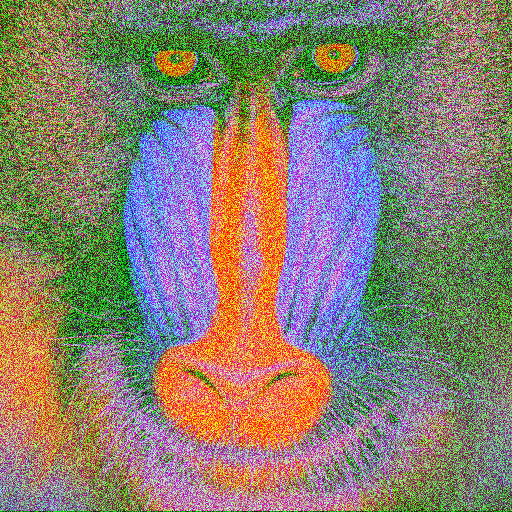
\includegraphics[height=.3\textwidth]{ps0-5-a-2.png}\\
	a&b\\
\end{tabular}
\end{center}
\caption{ 
\textit{a}. ps0-5-a-1 : Original Image 1  . \textit{b}. ps0-5-a-2 :  Image 1 with green noise. }
\label{ps0-5-a}
\end{figure}

\subsection{Noise introduction in the blue monochrome image}

 \begin{figure}[H]
\begin{center}
\begin{tabular}{cc}
	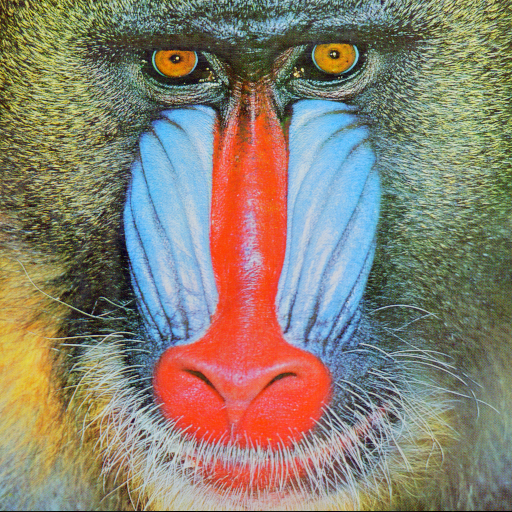
\includegraphics[height=.3\textwidth]{ps0-5-b-1.png}&
	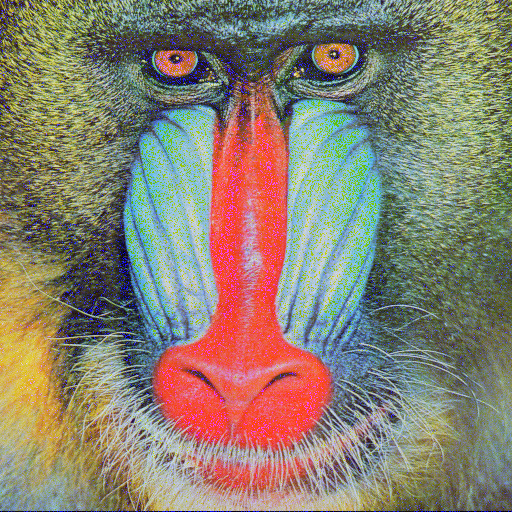
\includegraphics[height=.3\textwidth]{ps0-5-b-2.png}\\
	a&b\\
\end{tabular}
\end{center}
\caption{ 
\textit{a}. ps0-5-b-1 : Original Image 1  . \textit{b}. ps0-5-b-2 : Image 1 with blue noise. }
\label{ps0-5-b}
\end{figure}



\subsection{Comparison}

The blue version is well better than the green one. Indeed, the green noise can be observe instantaneously even with a small value of $\sigma$ whereas the blue noise must be really strong to be distinguish. As a matter of fact, the color to which the brain is the less sensitive is the blue so it seems logical that the value has to be increased a lot in order for us to see the impact.

\end{document}